\documentclass[ARTICLETHERMIC.tex]{subfiles}

\begin{document}

The algorithm described in this paper for filling the gaps in daily air temperature and total precipitation datasets is based on the implementation of the classical MLR method presented in \cite{eischeid_creating_2000}. The MLR method is a robust, efficient, accurate, and well known method that can indirectly account for local effects, such as topography, land cover, land use and surface water. While creating serially complete daily datasets of air temperature and total precipitation for the western U.S., \cite{eischeid_creating_2000} found that the MLR method consistently outperformed the other classical methods tested (normal ratio, inverse distance, optimal interpolation, and single best estimator). The same result was also found by \cite{xia_forest_1999} for a study in Bavaria, Germany. Moreover, in a study conducted in Iran for different climate conditions (dry to extra humid conditions), \cite{kashani_evaluation_2011} found that the estimation obtained with the MLR method compared well with those obtained with more recent methods, more specifically the artificial neural network (reference) and the genetic programming (references) techniques.

The algorithm that was developed in this work for filling the gaps in weather datasets is presented in the flowchart of \cref{fig:fillworker_flowchart}. It consists of two nested loops: the external `Loop A' iterates over the time series of four weather variables (min, max, and mean air temperature and total precipitation) for the target station while the inner `Loop B' iterates over every missing value in each data series. The estimation of a single missing value is achieved with a two-step procedure. The first step consists in selecting the data series with the best correlation coefficient, which also respect a certain number of conditions. The second step consists in building a MLR model and estimating the missing values. This is described in more details below.

\begin{figure}[!p]
    \centering
    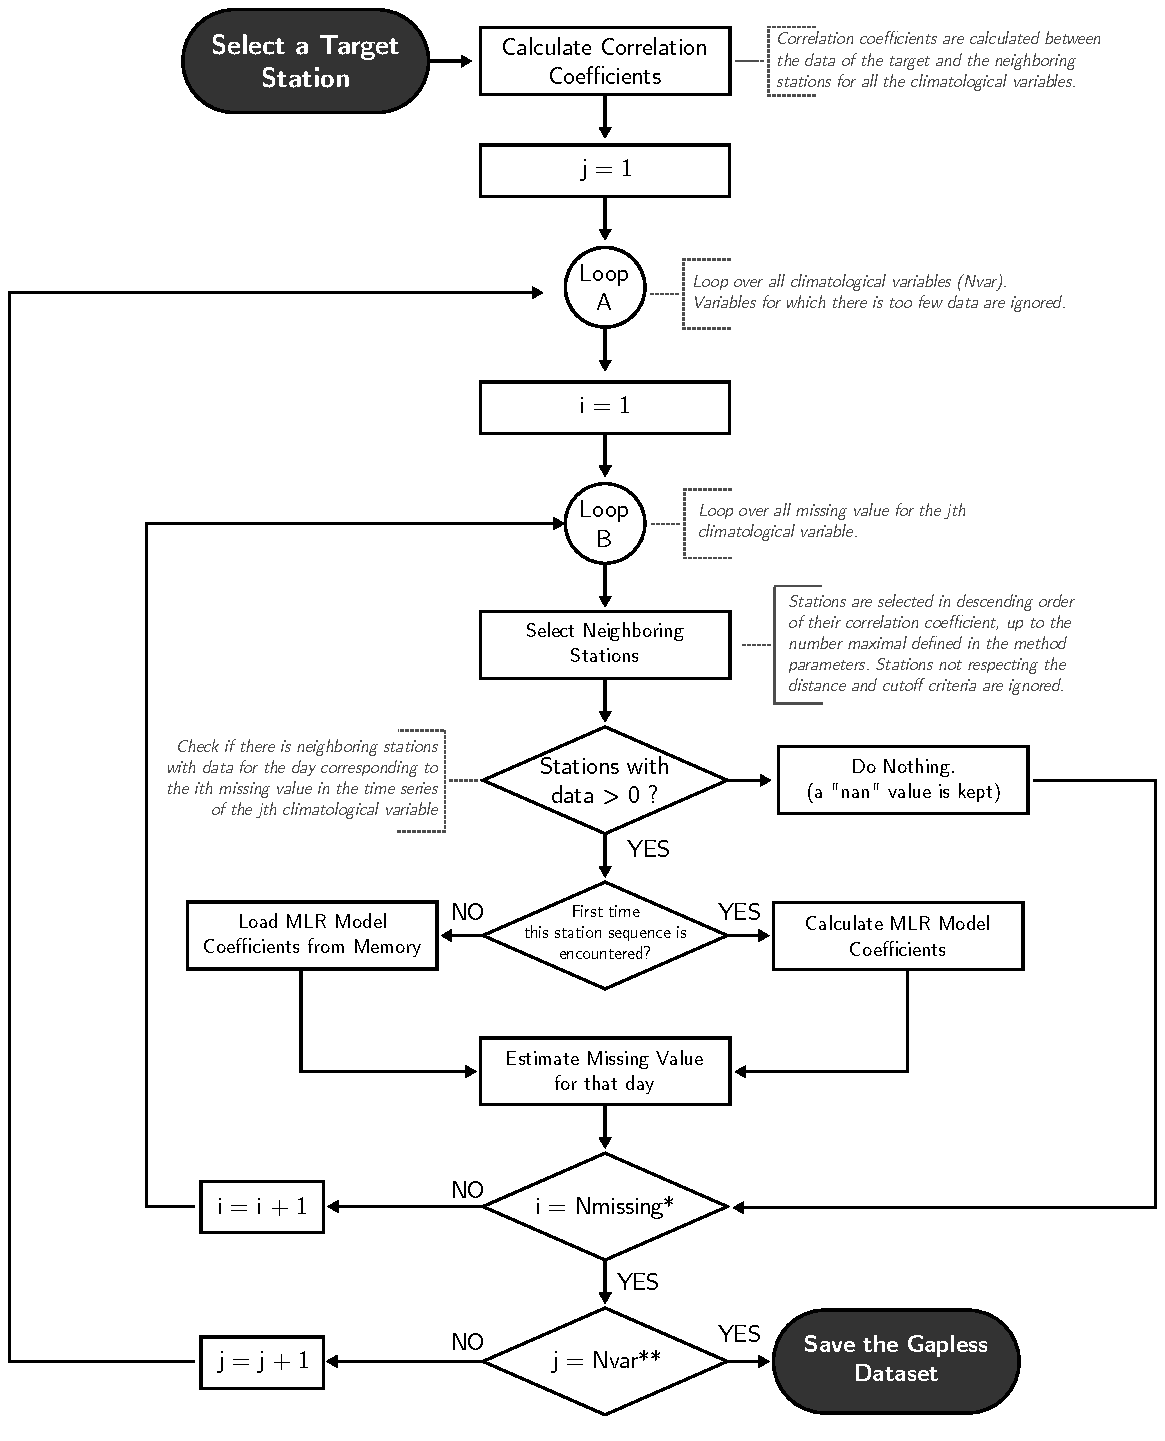
\includegraphics[width=\textwidth]{img/Flowchart-filling_missing_weather.pdf} 
    \caption{}
    \label{fig:fillworker_flowchart}
\end{figure}

\subsection{Loop A}

\subsubsection{Quality Control}

Prior to the analysis of weather time series, it is important to apply quality control constraints to ensure that the data do not violate obvious constraints associated with minimum, maximum, and average daily air temperature and daily cumulative precipitation. 

The program will identify irregularities or inconsistencies to insure that maximum, minimum and average daily temperatures are coherent for a given day and that all daily precipitation values are positive. Erroneous values are replaced by nan values in the dataset. These values will subsequently be estimated by the program from neighboring stations.

\subsubsection{Station Correlation Assessment}

The first step consists in calculating the correlation coefficients between data of the target station and those of the neighboring stations for each of the four weather variables: minimum, maximum and average daily temperatures and daily cumulative precipitation. These coefficients are calculated for the entire time-series for each neighboring station individually. If there are less than 182 synchronous values between the data of the target station and those of a neighboring station for a given variable, the correlation is not computed and a ‘‘NaN’’ value is kept instead.

\subsection{Loop B}

\subsubsection{Selection of the neighboring stations}

The selection of surrounding stations is critically important for the accurate estimation of missing weather data (Eischeid et al., 1995). Problems arise though because of synchronized missing values in the target and neighboring weather station datasets that varies trough time. This is illustrated in Table 8.1, where theoretical time-series of air temperature data with a realistic distribution of missing values are presented.

In \cref{tab:selectStations}, there are missing values in the target station dataset for days 2, 4, and 5. The missing value on day 2 will then be estimated with the data of the neighboring stations Y1, Y3, and Y4 since station Y2 is also missing a value on this day. All neighboring stations will be used for the estimation of the missing value on day 4, while only stations Y1 and Y2 have data available for the estimation of the missing value on day 5.

Data correlation between two stations will generally decreases as the horizontal and vertical distances increase. It is possible to specify a cutoff distance and a cutoff altitude difference for which neighboring stations that fall above these cutoff values are ignored by the program. The default values are set to 100 km and 350 m for the horizontal and vertical distance respectively based on the literature (Simolo et al., 2010; Tronci et al., 1986; Xia et al., 1999).

\begin{table}[!hb]
\newcommand{\nan}{\multicolumn{1}{c}{\textbf{nan}}}
\center
\caption{This table shows some data}
\begin{tabular}{
S[table-format = 1]
*5S[table-format = 2.1]
}
\toprule
& {Target} & \multicolumn{4}{c}{Neighbors} \\
\cmidrule(lr){3-6}
{Day} & {Y} & {X1} & {X2} & {X3} & {X4} \\
\midrule
%\rowcolor{gray!30}
1 & 11.0 & 12.0 & 12.0 & 12.5 & 10.0 \\
2 & \nan & 12.0 & \nan & 13.0 & 12.2 \\
3 &  7.5 &  8.5 &  8.5 &  8.0 &  8.9 \\
4 & \nan &  6.0 &  4.5 &  5.0 &  4.4 \\
5 & \nan &  8.0 &  8.5 & \nan & \nan \\
\bottomrule
\end{tabular}
\label{tab:selectStations}
\end{table}

Since the number of neighboring stations with available data is not fixed in time, it is not possible to use a single MLR model to fill all the missing values for the target station all at once. For each missing value in the target station dataset, the program keeps only the datasets of the neighboring stations that also have data at this particular time. Data series of stations that do not respect the cutoff criteria for distance and elevation differences are also ignored. Data from neighboring stations are selected in descending order of their correlation coefficient with the target station, up to a maximal number of stations defined in the method parameters. The default value for the maximal number of neighboring station was set to four, based on the literature (Eischeid et al., 1995; Xia et al., 1999).

If for a given day, no neighboring stations have a measured value to fill a gap in the target station dataset, no calculation is done and a ‘‘NaN’’ value is kept in the series instead and the program pass to the next missing value in the target series.

\end{document}

%Among these techniques, methods based on the use of data from neighboring stations are generally favored to within-station methods, i.e. those that only use data from the series being filled.

%have been proven to perform poorly compared to methods based on the use of data from neighboring stations for the reconstruction of daily precipitation time series (Eischeid et al., 1995; Kemp et al., 1983; Simolo et al., 2010).

%The creation of a serially complete weather dataset generally consists in the replacement of missing daily data with estimated values calculated from simultaneous observations at nearby stations. 

%Numerous spatial interpolation techniques exist for handling the missing data in the weather time series of a given station by using data from irregularly spaced neighboring station (e.g. simple arithmetic averaging, inverse distance method, single best estimator and multiple regression analysis).
